% Página
\section{Integridade}

A integridade trata da detecção de alterações indevidas nos dados. Funções de hash, MACs e assinaturas digitais podem apoiar essa verificação, mas oferecem garantias diferentes: um hash simples não autentica a origem, e seu uso para detectar adulteração deliberada depende de o resumo ser obtido por um meio confiável.
\subsection{Hash}

Um hash é uma função que transforma uma entrada de dados (que pode variar de alguns bytes a grandes volumes de dados) em uma saída de tamanho fixo, geralmente representada como uma sequência de caracteres alfanuméricos. Esta transformação é determinística, o que significa que a mesma entrada sempre produzirá a mesma saída.\\

Alguns exemplos de algoritmos hash populares incluem a família de algoritmos SHA-2 (Secure Hash Algorithm 2), que inclui SHA-224, SHA-256, SHA-384 e SHA-512. Os algoritmos SHA-2 produzem hashes de diferentes tamanhos, sendo o SHA-256 e o SHA-512 os mais comuns, gerando valores de 256 e 512 bits, respectivamente.\\

A Figura \ref{fig:hash} mostra Bob enviando a mensagem e seu resumo para Alice. Ela calcula o resumo da mensagem recebida e compara os dois valores.\\

\begin{figure}[H]
	\centering
	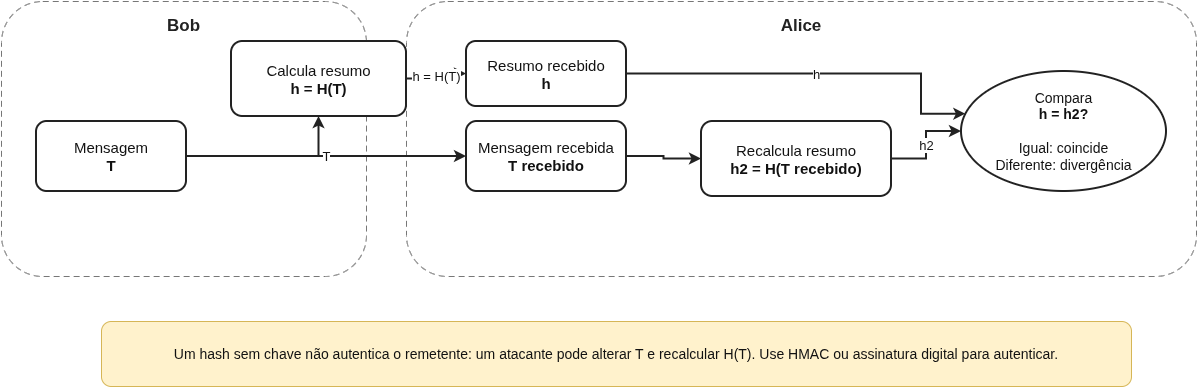
\includegraphics[scale=0.45]{hash.png}
	\caption{Comparação de resumos para detectar divergências em uma mensagem}
	\label{fig:hash}
\end{figure}

Bob calcula \(h=H(T)\) e envia a mensagem \(T\) junto com o resumo \(h\). Alice calcula \(h_2=H(T_{\mathrm{recebido}})\) sobre a mensagem recebida e compara \(h_2\) com \(h\). Se forem diferentes, a mensagem recebida diverge daquela que corresponde ao resumo. Se forem iguais, isso apenas indica que a mensagem coincide com o resumo recebido; um hash simples enviado junto com a mensagem não impede que um atacante altere ambos e recalcule o resumo. Para autenticar a origem e proteger contra adulteração deliberada, use um HMAC com segredo compartilhado ou uma assinatura digital cuja chave pública de Bob seja autenticada. O hash não cifra a mensagem.\\

\textbf{Prático}\\

O OpenSSL calcula resumos SHA-256 e SHA-512. Para comparar um arquivo com um resumo salvo, obtenha esse resumo por um meio confiável: se um atacante puder substituir tanto o arquivo quanto o resumo, a comparação não detectará a adulteração.

\begin{enumerate}
	\item Salvar o resumo SHA-256 de \texttt{arquivo.txt}. O resumo de referência precisa vir de uma fonte confiável.
	\begin{tcolorbox}[width=\textwidth]
	{\small
		\begin{verbatim}
		$ openssl dgst -sha256 arquivo.txt | awk '{print $NF}' > hash.sha256
		\end{verbatim}
	}
	\end{tcolorbox}

	\item Comparar o resumo atual de \texttt{arquivo.txt} com o resumo SHA-256 salvo.
	\begin{tcolorbox}[width=\textwidth]
	{\small
		\begin{verbatim}
		$ openssl dgst -sha256 arquivo.txt | awk '{print $NF}' | \
		  cmp -s - hash.sha256 && echo "Resumo igual" || \
		  { echo "Resumo divergente" >&2; exit 1; }
		\end{verbatim}
	}
	\end{tcolorbox}

	\item Salvar o resumo SHA-512 de \texttt{arquivo.txt}. O resumo de referência precisa vir de uma fonte confiável.
	\begin{tcolorbox}[width=\textwidth]
	{\small
		\begin{verbatim}
		$ openssl dgst -sha512 arquivo.txt | awk '{print $NF}' > hash.sha512
		\end{verbatim}
	}
	\end{tcolorbox}

	\item Comparar o resumo atual de \texttt{arquivo.txt} com o resumo SHA-512 salvo.
	\begin{tcolorbox}[width=\textwidth]
	{\small
		\begin{verbatim}
		$ openssl dgst -sha512 arquivo.txt | awk '{print $NF}' | \
		  cmp -s - hash.sha512 && echo "Resumo igual" || \
		  { echo "Resumo divergente" >&2; exit 1; }
		\end{verbatim}
	}
	\end{tcolorbox}
\end{enumerate}

\pagebreak
